\documentclass[12pt]{article}
\usepackage{graphicx}
\usepackage {color}
\usepackage{pdfpages}
\usepackage{float}
\usepackage{changebar}
\usepackage{enumitem,amssymb}
\renewcommand{\familydefault}{\sfdefault}
\usepackage[margin=1.2in]{geometry}
\usepackage{graphicx}
\usepackage{wrapfig}
\usepackage[super]{cite}
\usepackage{subcaption}
\usepackage[table]{xcolor}
\usepackage{amsmath}
\usepackage[sort, numbers]{natbib}
\usepackage{multirow}
\usepackage{tabularx}
\usepackage{siunitx}
\usepackage{matlab-prettifier}
\usepackage{wrapfig,lipsum,booktabs}
%%%%%%%%%%%%Defining the margins %%%%%%%%%%%%%%%%%%%%%
\textheight 9.in
\textwidth 6.5in
\topmargin -.5in
\oddsidemargin 0in
\setlength{\parskip}{\smallskipamount}

%%%%%%%%%%%%%%Specific Commands %%%%%%%%%%%%%%%%%%
\newcommand{\eg}{{\em e.g.,}}
\newcommand{\ie}{{\em i.e.,}}
\newcommand{\etc}{{\em etc.,}}
\newcommand{\etal}{{\em et al.}}
\newcommand{\degrees}{{$^{\circ}$}}
\newcommand{\fig}[1]{\textbf{Figure #1}}

%%%%%%%%%%%%%%%%%%%%%%%%%%%% Setting to control figure placement
% These determine the rules used to place floating objects like figures 
% They are only guides, but read the manual to see the effect of each.
\renewcommand{\topfraction}{.9}
\renewcommand{\bottomfraction}{.9}
\renewcommand{\textfraction}{.1}
\renewcommand{\familydefault}{\sfdefault} %setting the san serif font

%%%%%%%%%%%%%%%%%%%%%%%% Line spacing
% Use the following command for ``double'' spacing
%\setlength{\baselineskip}{1.2\baselineskip}
% and this one for an acceptable NIH spacing of 6lpi based on 11pt
%\setlength{\baselineskip}{.9\baselineskip}
% The baselineskip does not appear to work when we include a maketitle
% command in the main file.  Something there must set the line spacing
% If we use this next command, then things seem to work.
\renewcommand{\baselinestretch}{.9}

\setcounter{secnumdepth}{0} %make no numbers but have a table of contents


\begin{document}

\title{HW 4: Medical Imaging Systems}
\author{Jake Bergquist, u6010393 }
\maketitle

\section{Q1}
\noindent\textbf{a: } 
Attached is the drawn sinogram for (a). All of the profiles are either semicircular or semi oval with a smooth transition between the different angles.

\noindent\textbf{b: } 
Attached is the drawn sinogram

\section{Q2}
\noindent\textbf{a: } 


\noindent\textbf{b: }


\section{Q3}


\section{Q4}

\section{Q5}


\begin{figure}[H]

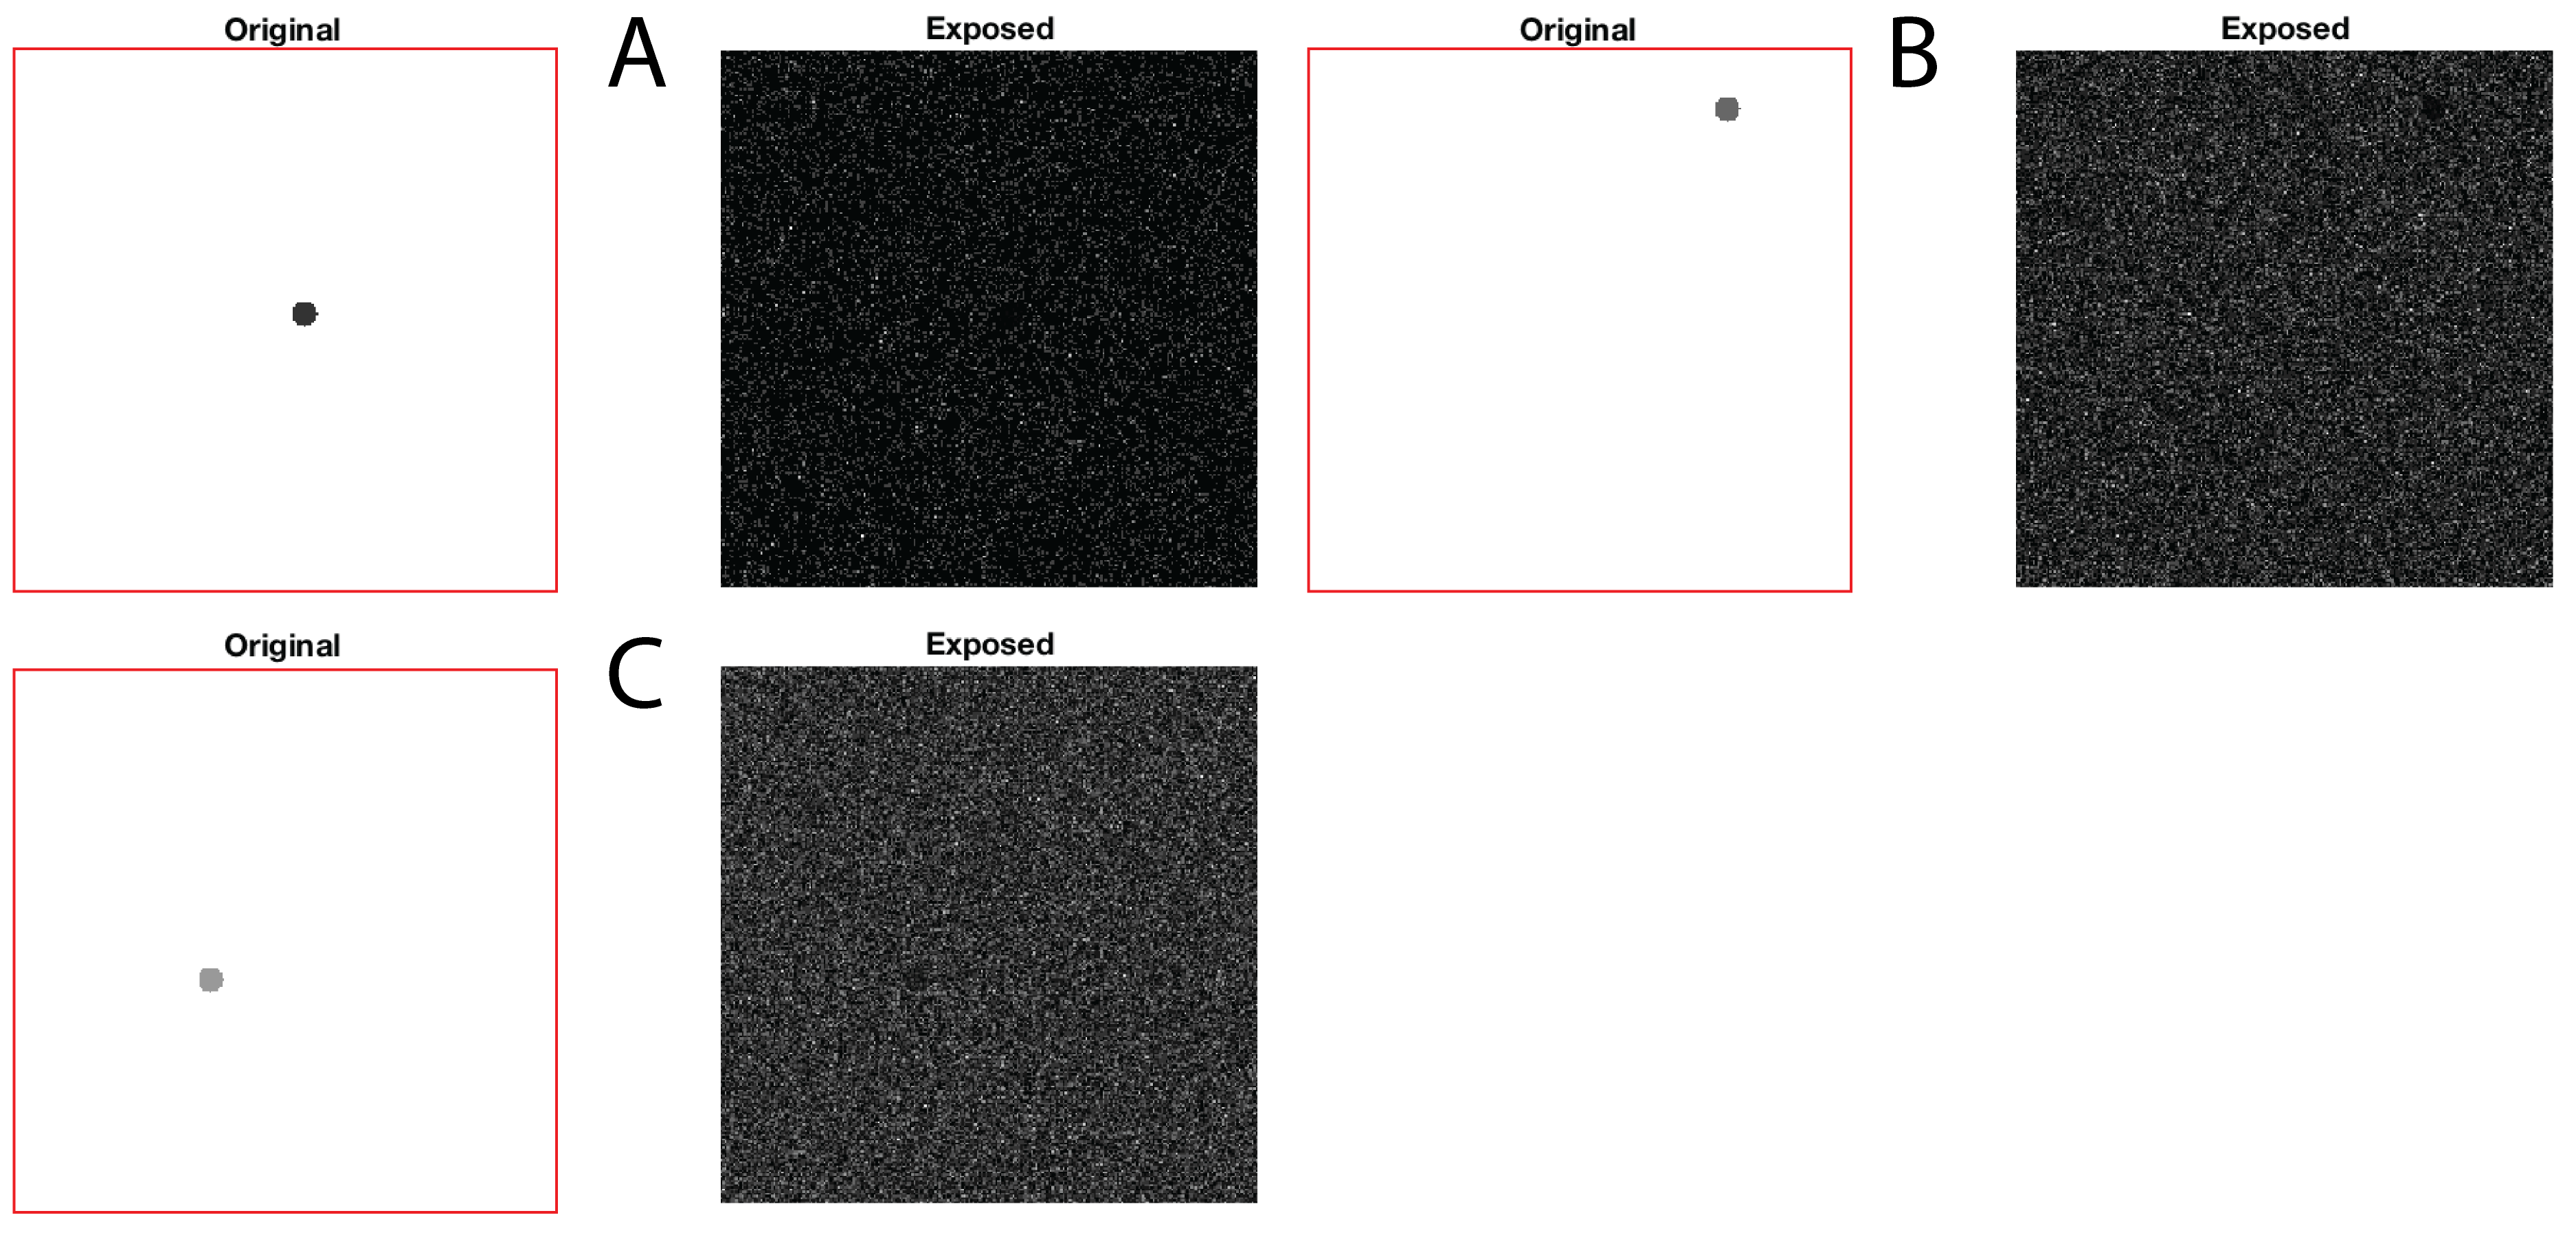
\includegraphics[width=\textwidth]{Figures/Obs1_fig.png}
\caption{Observer 1 minimum Lambda images: The original and exposed images for each intensity corresponding to the minimum lambda value at which the observer was able to detect a circle. A) the images for intensity of 0.2, lambda 0.2, B) intensity 0.4, lambda 1, D) intensity 0.6, lambda 2. This observer could not detect a circle at intensity 0.8 for any lambda value used.}
\label{Fig:obs1Img}
\end{figure}



\begin{lstlisting}[style=Matlab-editor]
%%


\end{lstlisting}

\end{document}



\begin{figure}[H]
	\centering
	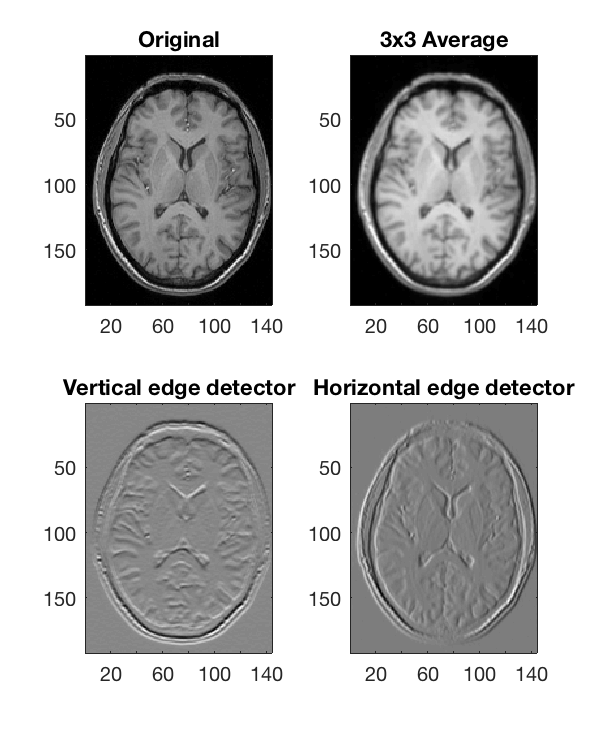
\includegraphics[width=\textwidth]{Figures/convs.png}
	\caption{}
	\label{Fig:conv}
\end{figure}

\begin{lstlisting}[style=Matlab-editor]

\end{lstlisting}




